\documentclass[12pt,ngerman,parskip=half]{scrartcl}

\usepackage{babel}
\usepackage{blindtext}
\usepackage{graphicx}
\usepackage[utf8]{inputenc}

\author{Uwe Ziegenhagen}
\title{Mein erstes LaTeX-Dokument}
\date{Köln, den \today} % leerlassen zum Unterdrücken

\begin{document}
\maketitle

\tableofcontents

\listoffigures

\section{Einführung}
\subsection{Literaturüberblick}
\subsubsection{Deutsche Literatur}

Wie wir in Abschnitt \ref{sec:ausblick} sehen werden...

Hallo Fernuni!
Ich bin ein einfacher Text.

Um einen neuen Absatz zu beginnen, fügen wir einfach eine Leerzeile ein.

% Formate png, pdf, jpg

% h = here, t = top, b = bottom, p = eigene Seite, !

\begin{figure}[b] % float, htbp!
\begin{center}

\includegraphics[width=10cm]{Bilder/Katze}
\end{center}
\caption{Katze 1}\label{fig:katze}
\end{figure}

\blindtext[1]


\begin{figure}[h]
\begin{center}

\includegraphics[width=0.8\textwidth]{Bilder/miau}
\end{center}
\caption{Katze 2}\label{fig:miau}
\end{figure}

\blindtext[5]


\begin{figure}[b]
\begin{center}
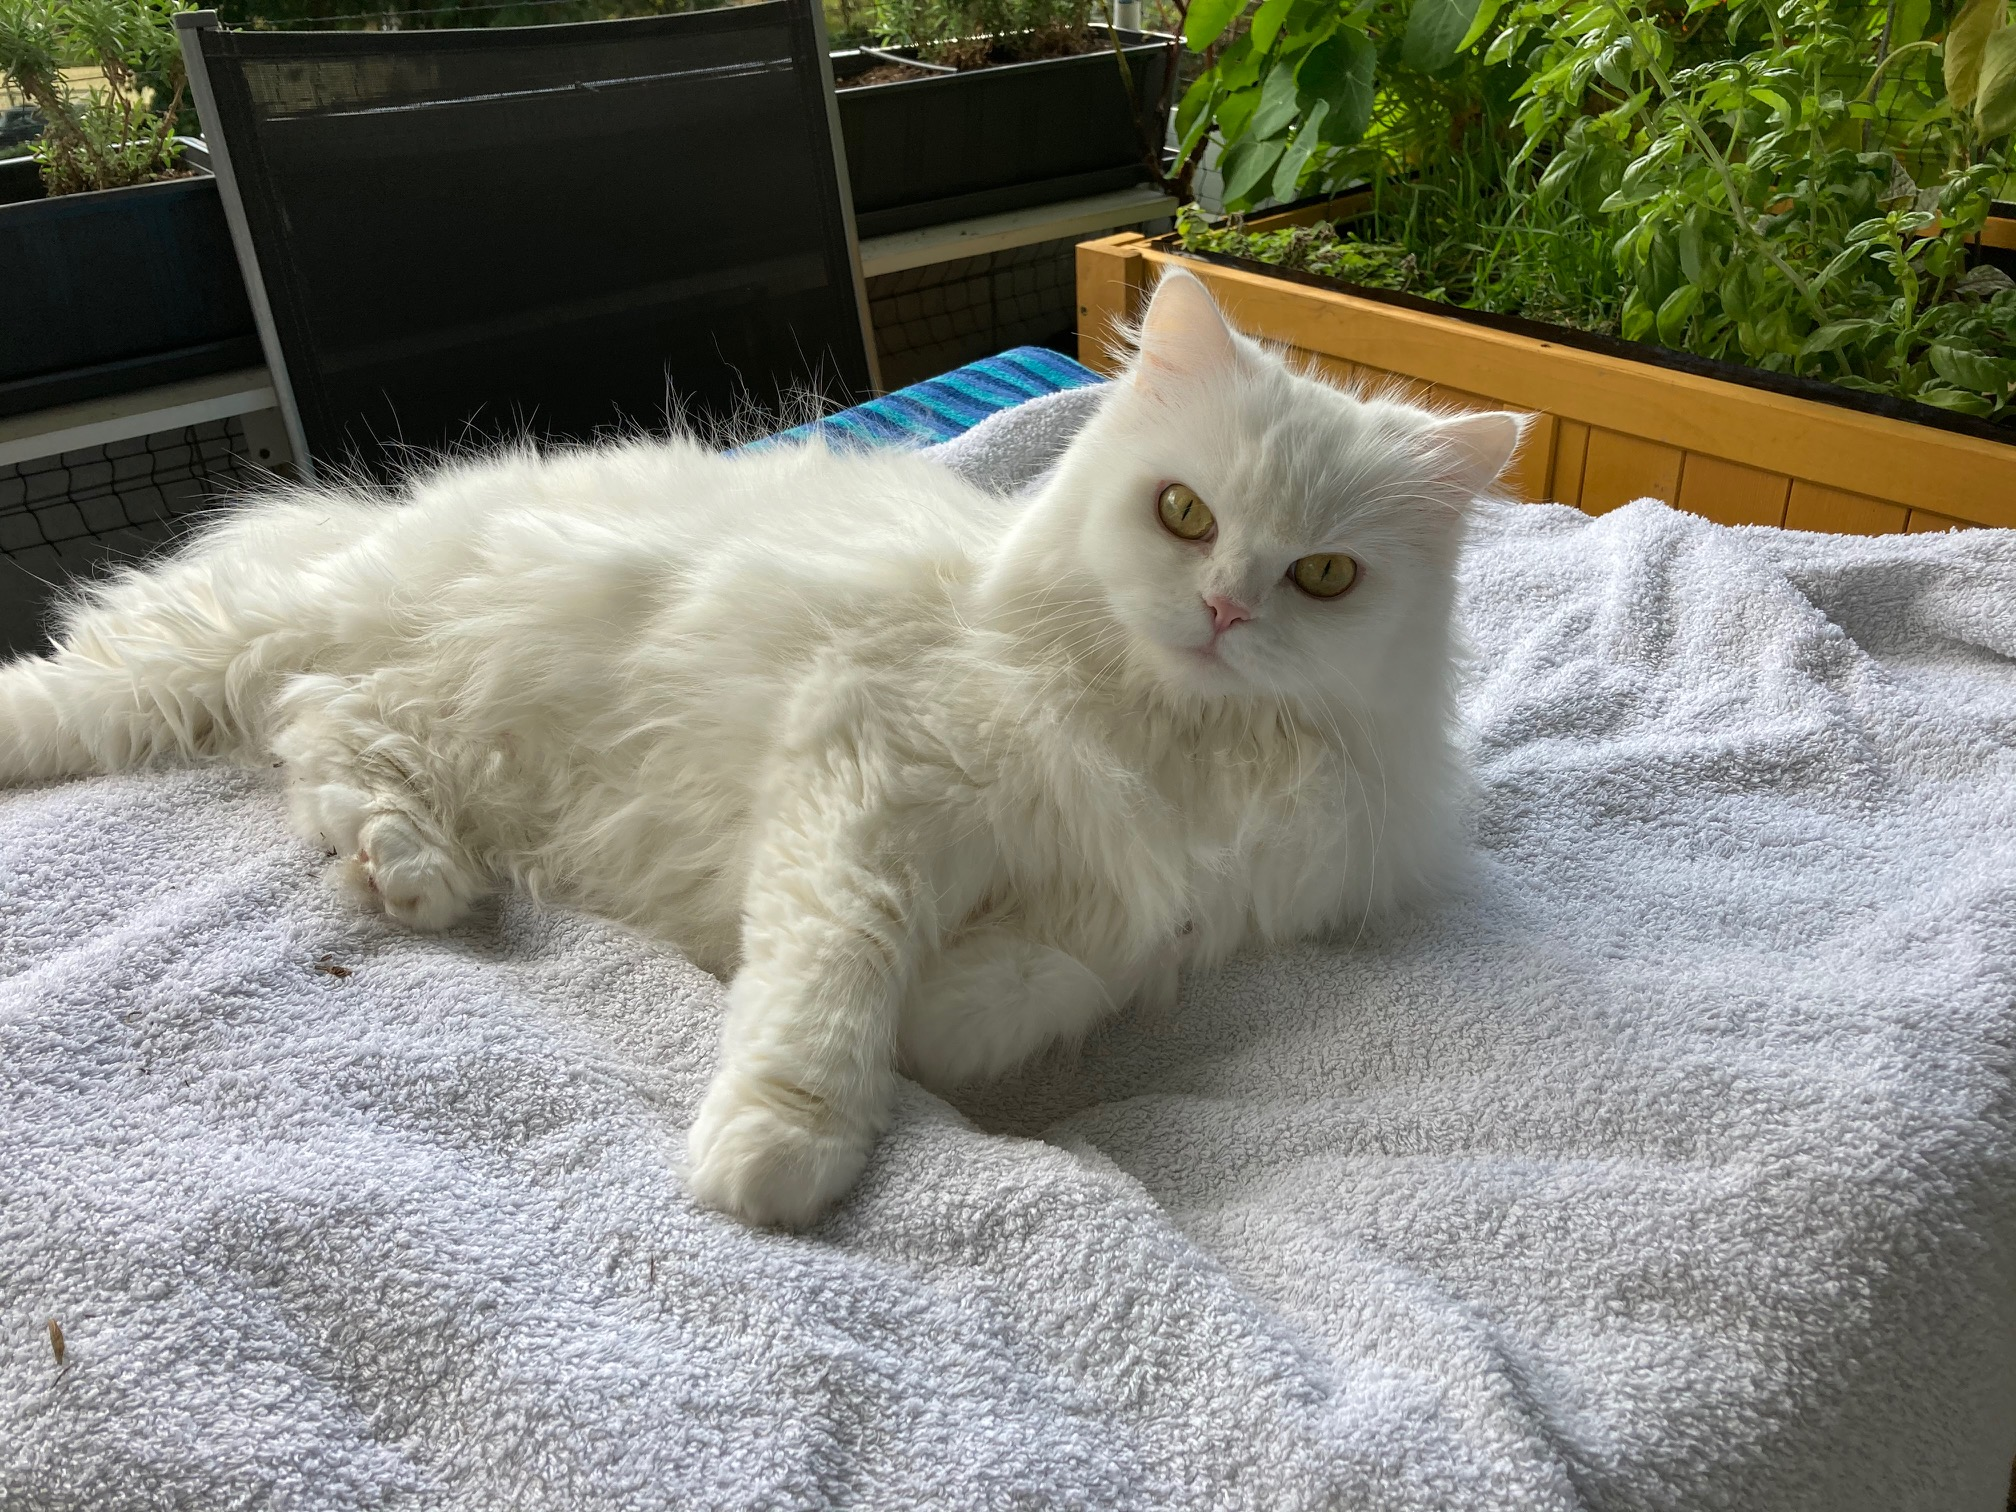
\includegraphics[width=\textwidth]{Bilder/Katze1}
\end{center}
\caption{Katze 3}\label{fig:katze1}
\end{figure}

\blindtext[5]

\section{fdsdfsd}
\subsection{fsdfsdfs}
\subsubsection{Internationale Forschung}

\blindtext

\paragraph{sdfsdf} \blindtext

\subparagraph{sdfsdf} \blindtext


\section{Analyse}

\blindtext[5]

%\pagebreak
\section{Fazit}

\subsection{Ausblick}\label{sec:ausblick} 

Siehe Abbildung \ref{fig:katze} auf Seite \pageref{fig:katze}

\begin{center}

\includegraphics[width=\textwidth]{Bilder/Katze}
\end{center}
\captionof{figure}{Katze 4}\label{fig:katze2}


\blindtext

\"a

%ert etr er t 
\includegraphics[width=2mm]{Bilder/Katze} trreterte

öäöäöäöäöä

\end{document}




